\documentclass[11pt,a4paper]{report}

\usepackage[utf8]{inputenc}
\usepackage[T1]{fontenc}
\usepackage[margin=1in]{geometry}
\usepackage{graphicx}
\usepackage{xcolor}
\usepackage{listings}
\usepackage{hyperref}
\usepackage{booktabs}
\usepackage{enumitem}
\usepackage{fancyhdr}
\usepackage{titlesec}
\usepackage{tocloft}
\usepackage{amsmath}
\usepackage{tikz}
\usepackage{multicol}
\usepackage{float}
\usepackage{longtable}

% Colors
\definecolor{codebackground}{RGB}{245,245,245}
\definecolor{codecomment}{RGB}{0,128,0}
\definecolor{codekeyword}{RGB}{0,0,180}
\definecolor{codestring}{RGB}{163,21,21}
\definecolor{linkcolor}{RGB}{0,80,160}
\definecolor{chaptercolor}{RGB}{40,60,100}
\definecolor{relayblue}{RGB}{65,105,225}
\definecolor{relaygreen}{RGB}{60,160,60}
\definecolor{relayorange}{RGB}{220,130,50}
\definecolor{relayred}{RGB}{190,60,60}

\hypersetup{
    colorlinks=true,
    linkcolor=linkcolor,
    urlcolor=linkcolor,
    citecolor=linkcolor,
    pdftitle={Zend Relay Software Documentation},
    pdfauthor={Strydr Silverberg},
}

\lstdefinestyle{codestyle}{
    backgroundcolor=\color{codebackground},
    basicstyle=\ttfamily\small,
    breakatwhitespace=false,
    breaklines=true,
    captionpos=b,
    commentstyle=\color{codecomment}\itshape,
    keywordstyle=\color{codekeyword}\bfseries,
    stringstyle=\color{codestring},
    numberstyle=\tiny\color{gray},
    numbers=left,
    numbersep=8pt,
    showspaces=false,
    showstringspaces=false,
    showtabs=false,
    tabsize=4,
    frame=single,
    framerule=0.5pt,
    rulecolor=\color{gray!50},
}
\lstset{style=codestyle}

\titleformat{\chapter}[display]
    {\normalfont\huge\bfseries\color{chaptercolor}}
    {\chaptertitlename\ \thechapter}{20pt}{\Huge}
\titlespacing*{\chapter}{0pt}{0pt}{30pt}

\pagestyle{fancy}
\fancyhf{}
\fancyhead[L]{\leftmark}
\fancyhead[R]{\thepage}
\renewcommand{\headrulewidth}{0.4pt}
\setlength{\headheight}{14pt}

\newcommand{\notebox}[1]{%
    \begin{center}
    \fcolorbox{gray}{gray!10}{%
        \parbox{0.9\textwidth}{\textbf{Note:} #1}
    }
    \end{center}
}

\newcommand{\warningbox}[1]{%
    \begin{center}
    \fcolorbox{red!70}{red!10}{%
        \parbox{0.9\textwidth}{\textbf{Warning:} #1}
    }
    \end{center}
}

\newcommand{\tipbox}[1]{%
    \begin{center}
    \fcolorbox{green!60!black}{green!5}{%
        \parbox{0.9\textwidth}{\textbf{Tip:} #1}
    }
    \end{center}
}

\title{%
    \vspace{-1cm}
    \rule{\textwidth}{1pt}\\[0.5cm]
    {\Huge\bfseries Zend}\\[0.3cm]
    {\Large Relay Software Documentation}\\[0.3cm]
    \rule{\textwidth}{1pt}\\[1cm]
    {\large Architecture, API, packet handling, storage, and operational behavior}
}
\author{Strydr Silverberg}
\date{\today}

\begin{document}

\maketitle
\thispagestyle{empty}

\vfill
\begin{center}
    \textit{A complete technical guide to the Zend relay server, including request flow,\
    blob lifecycle, runtime configuration, rate limiting, cleanup, and encrypted packet framing.}
\end{center}
\vfill

\newpage
\tableofcontents
\newpage

%==============================================================================
\chapter{Overview}
%==============================================================================

\section{What the Relay Does}

The Zend relay is a lightweight HTTP service written in Zig that accepts encrypted uploads, stores them temporarily on disk, and serves each uploaded blob back exactly once. The relay is intentionally narrow in scope: it does not perform encryption, key derivation, or plaintext inspection. Instead, it stores opaque ciphertext produced by the sender and deletes the stored blob after download or expiration.

At a high level, the relay is responsible for four jobs:

\begin{enumerate}
    \item \textbf{Session creation} --- issue an upload ID and upload token.
    \item \textbf{Chunk intake} --- append encrypted frame data to a temporary file in order.
    \item \textbf{Finalization and serving} --- atomically promote the completed upload and later return it to a downloader.
    \item \textbf{Lifecycle management} --- enforce size limits, rate limits, and time-to-live cleanup.
\end{enumerate}

\section{Design Goals}

The implementation in the provided source files suggests a relay designed around the following goals:

\begin{itemize}[leftmargin=1.5cm]
    \item \textbf{Simplicity} --- plain file-backed storage instead of a database.
    \item \textbf{Opaque transport} --- the server handles ciphertext blobs without needing the file key.
    \item \textbf{Streaming-friendly uploads} --- upload data arrives as ordered append requests rather than a single giant POST.
    \item \textbf{Short-lived storage} --- completed and abandoned uploads are automatically reaped.
    \item \textbf{Small trusted computing base} --- the relay mostly validates ordering, authorization, sizes, and file state.
\end{itemize}

\section{System Architecture}

\begin{center}
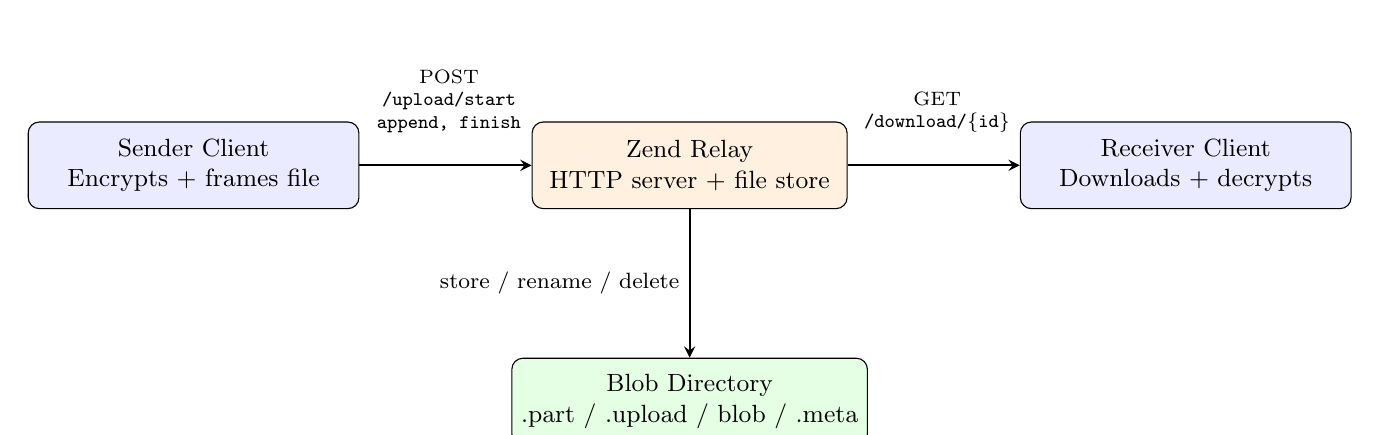
\begin{tikzpicture}[
    box/.style={draw, rounded corners, minimum width=3.4cm, minimum height=1.1cm, align=center, font=\small},
    arr/.style={->, thick, >=stealth}
]
    \node[box, fill=blue!8, minimum width=4.2cm] (sender) at (-6.3,0) {Sender Client\\Encrypts + frames file};
    \node[box, fill=orange!12, minimum width=4.0cm] (relay) at (0,0) {Zend Relay\\HTTP server + file store};
    \node[box, fill=green!10, minimum width=4.2cm] (disk) at (0,-3) {Blob Directory\\.part / .upload / blob / .meta};
    \node[box, fill=blue!8, minimum width=4.2cm] (receiver) at (6.3,0) {Receiver Client\\Downloads + decrypts};

    \draw[arr] (sender) -- node[pos=0.52, above=10pt, align=center, font=\scriptsize, fill=white, inner sep=1.5pt] {POST\\\texttt{/upload/start}\\\texttt{append, finish}} (relay);
    \draw[arr] (relay) -- node[left,font=\footnotesize] {store / rename / delete} (disk);
    \draw[arr] (relay) -- node[pos=0.52, above=10pt, align=center, font=\scriptsize, fill=white, inner sep=1.5pt] {GET\\\texttt{/download/\{id\}}} (receiver);
\end{tikzpicture}
\end{center}


\section{Source Files Covered}

This document is based on the relay-related source files currently available:

\begin{longtable}{ll}
\toprule
\textbf{File} & \textbf{Role} \\
\midrule
\texttt{main.zig} & Listener setup, connection loop, route dispatch,\\
\texttt{} & CORS preflight, thread spawning \\
\texttt{runtime\_config.zig} & Environment-variable based runtime configuration \\
\texttt{config.zig} & Default limits and timings \\
\texttt{http\_helpers.zig} & Request body reading and plain-text responses \\
\texttt{upload.zig} & Upload start, append, and finish endpoints \\
\texttt{download.zig} & Download endpoint with consume-on-read deletion \\
\texttt{delete.zig} & Token-protected blob deletion endpoint \\
\texttt{storage.zig} & Path construction and file cleanup helpers \\
\texttt{rate\_limit.zig} & Per-IP request accounting and route-aware quotas \\
\texttt{reaper.zig} & Expiration of complete and incomplete uploads \\
\texttt{ids.zig} & Random hexadecimal IDs and identifier validation \\
\texttt{blob\_format.zig} & Encrypted frame format and stream parser helpers \\
\texttt{packet\_types.zig} & Packet type and framing constants \\
\texttt{aead.zig}, \texttt{chacha20.zig}, \texttt{poly1305.zig} & Authenticated encryption implementation used \\
\texttt{} & by the protocol \\
\bottomrule
\end{longtable}

\notebox{The relay itself primarily stores and serves opaque bytes. The packet-format and AEAD files are still included here because they define the blob structure that the relay transports and the clients later decrypt.}

%==============================================================================
\chapter{Build-Time Defaults and Runtime Configuration}
%==============================================================================

\section{Default Configuration}

The relay ships with a small set of hard-coded defaults in \texttt{config.zig}:

\begin{table}[H]
\centering
\begin{tabular}{lll}
\toprule
\textbf{Name} & \textbf{Default} & \textbf{Meaning} \\
\midrule
\texttt{DEFAULT\_PORT} & 8080 & HTTP listen port \\
\texttt{BLOB\_DIR} & \texttt{blobs} & Directory used for blob and metadata files \\
\texttt{MAX\_UPLOAD\_SIZE} & 512 MiB & Maximum completed blob size \\
\texttt{MAX\_APPEND\_BODY\_SIZE} & 1 MiB & Maximum body accepted by one append \\
\texttt{} & & request \\
\texttt{TTL\_SECONDS} & 24 hours & Lifetime of a completed uploaded blob \\
\texttt{INCOMPLETE\_TTL\_SECONDS} & 1 hour & Lifetime of abandoned partial uploads \\
\texttt{REAP\_INTERVAL\_NS} & 60 seconds & Background cleanup interval \\
\texttt{RATE\_LIMIT\_WINDOW\_SECONDS} & 60 & Rate-limit window size \\
\texttt{RATE\_LIMIT\_MAX\_REQUESTS\_PER\_IP} & 240 & Total requests per IP per window \\
\texttt{RATE\_LIMIT\_MAX\_UPLOAD\_STARTS\_PER\_IP} & 20 & Upload session creations per window \\
\texttt{RATE\_LIMIT\_MAX\_UPLOAD\_APPENDS\_PER\_IP} & 1200 & Chunk append requests per window \\
\texttt{RATE\_LIMIT\_MAX\_UPLOAD\_FINISHES\_PER\_IP} & 40 & Upload finalizations per window \\
\texttt{RATE\_LIMIT\_MAX\_DOWNLOADS\_PER\_IP} & 120 & Download requests per window \\
\bottomrule
\end{tabular}
\caption{Relay defaults from \texttt{config.zig}}
\end{table}

\section{Environment Variables}

The relay resolves its runtime behavior from environment variables in \texttt{runtime\_config.zig}. Each variable falls back to the default above when unset.

\begin{table}[H]
\centering
\begin{tabular}{ll}
\toprule
\textbf{Environment Variable} & \textbf{Purpose} \\
\midrule
\texttt{ZEND\_RELAY\_HOST} & Bind host string \\
\texttt{ZEND\_RELAY\_PORT} & Bind port \\
\texttt{ZEND\_BLOB\_DIR} & Blob directory path \\
\texttt{ZEND\_MAX\_UPLOAD\_BYTES} & Total allowed blob size \\
\texttt{ZEND\_MAX\_APPEND\_BODY\_BYTES} & Maximum append request size \\
\texttt{ZEND\_TTL\_SECONDS} & Completed blob lifetime \\
\texttt{ZEND\_INCOMPLETE\_TTL\_SECONDS} & Partial upload lifetime \\
\texttt{ZEND\_ALLOWED\_ORIGINS} & CORS \texttt{Access-Control-Allow-Origin} value \\
\texttt{ZEND\_RATE\_LIMIT\_WINDOW\_SECONDS} & Rate-limit window length \\
\texttt{ZEND\_RATE\_LIMIT\_MAX\_REQUESTS\_PER\_IP} & Total request cap \\
\texttt{ZEND\_RATE\_LIMIT\_MAX\_UPLOAD\_STARTS\_PER\_IP} & Start cap \\
\texttt{ZEND\_RATE\_LIMIT\_MAX\_UPLOAD\_APPENDS\_PER\_IP} & Append cap \\
\texttt{ZEND\_RATE\_LIMIT\_MAX\_UPLOAD\_FINISHES\_PER\_IP} & Finish cap \\
\texttt{ZEND\_RATE\_LIMIT\_MAX\_DOWNLOADS\_PER\_IP} & Download cap \\
\bottomrule
\end{tabular}
\caption{Runtime environment variables}
\end{table}

\section{Startup Sequence}

When \texttt{main()} runs, it performs the following initialization sequence:

\begin{enumerate}
    \item Create a general-purpose allocator.
    \item Load runtime config from the environment.
    \item Ensure the blob directory exists with \texttt{makePath()}.
    \item Initialize the in-memory rate limiter.
    \item Bind a TCP listener on \texttt{0.0.0.0:\{port\}}.
    \item Spawn the background reaper thread.
    \item Accept incoming TCP connections forever, creating a worker thread per connection.
\end{enumerate}

At startup the relay logs the listen address, blob directory, upload limit, blob TTL, and rate-limit settings. This gives a concise operational snapshot in systemd logs.

%==============================================================================
\chapter{HTTP Server Structure}
%==============================================================================

\section{Connection Handling}

Each accepted TCP connection is passed to \texttt{handleConnection()}, which constructs a Zig HTTP server around the connection stream and then processes requests in a loop until the client closes the connection.

Within that loop, the relay:

\begin{enumerate}
    \item Parses the request head.
    \item Normalizes the path by stripping any query string.
    \item Logs the client IP, HTTP method, and request path.
    \item Handles CORS \texttt{OPTIONS} requests immediately.
    \item Applies per-IP rate limiting based on the classified route.
    \item Dispatches to the upload, download, or delete handler.
    \item Falls back to \texttt{404 Not found} for unknown paths.
\end{enumerate}

\section{Client IP Extraction}

The relay derives an IP string from the accepted socket address using \texttt{clientIpString()}. The helper formats the address, then trims brackets for IPv6 and trims the final port component for IPv4-style \texttt{host:port} strings.

This string becomes the lookup key for rate limiting and is also included in request logs.

\section{Route Classification}

Before rate limiting, the relay maps each path to a route class:

\begin{table}[H]
\centering
\begin{tabular}{ll}
\toprule
\textbf{Path Pattern} & \textbf{Route Kind} \\
\midrule
\texttt{/upload/start} & \texttt{upload\_start} \\
\texttt{/upload/append/...} & \texttt{upload\_append} \\
\texttt{/upload/finish/...} & \texttt{upload\_finish} \\
\texttt{/download/...} & \texttt{download} \\
anything else & \texttt{other} \\
\bottomrule
\end{tabular}
\caption{Route classes used by the rate limiter}
\end{table}

\section{CORS Behavior}

The relay handles CORS in two places:

\begin{itemize}[leftmargin=1.5cm]
    \item In \texttt{main.zig}, an \texttt{OPTIONS} request receives a \texttt{204 No Content} response with allow-origin, allow-methods, and allow-headers.
    \item Normal endpoint responses include \texttt{Access-Control-Allow-Origin} through \\\texttt{http\_helpers.respondText()} or route-specific JSON/binary responses.
\end{itemize}

The allowed origin is not dynamically echoed from the request. Instead, it is emitted directly from \texttt{cfg.allowed\_origins}. This keeps behavior simple, but it also means deployments need to set that value correctly for the web frontend.

%==============================================================================
\chapter{Upload Flow}
%==============================================================================

\section{Overview}

Uploads are split into three HTTP actions:

\begin{enumerate}
    \item \texttt{POST /upload/start}
    \item \texttt{POST /upload/append/\{id\}?token=...\&index=N}
    \item \texttt{POST /upload/finish/\{id\}?token=...}
\end{enumerate}

The relay stores upload state in two files during the transfer:

\begin{itemize}[leftmargin=1.5cm]
    \item \texttt{\{id\}.part} --- partial ciphertext bytes
    \item \texttt{\{id\}.upload} --- token, creation time, next expected chunk index, bytes written
\end{itemize}

This lets the relay remain stateless across requests except for the filesystem.

\section{Upload Start}

\subsection{Endpoint}

\begin{lstlisting}[language=bash]
POST /upload/start
\end{lstlisting}

\subsection{Behavior}

\texttt{handleStart()} creates a new upload session as follows:

\begin{enumerate}
    \item Reject any method other than \texttt{POST}.
    \item Generate a random 16-character hexadecimal upload ID.
    \item Generate a separate random 16-character hexadecimal upload token.
    \item Create an empty temporary blob file \texttt{\{id\}.part}.
    \item Create an upload state file \texttt{\{id\}.upload} initialized with:
    \begin{itemize}
        \item token
        \item creation timestamp
        \item next expected append index = 0
        \item bytes written = 0
    \end{itemize}
    \item Return JSON containing the ID and token.
\end{enumerate}

\subsection{Response Shape}

\begin{lstlisting}[language={}]
{"id":"<upload-id>","token":"<upload-token>"}
\end{lstlisting}

\section{Upload Append}

\subsection{Endpoint}

\begin{lstlisting}[language=bash]
POST /upload/append/{id}?token=<token>&index=<n>
\end{lstlisting}

\subsection{Expected Client Behavior}

Each append request contains one encrypted frame or a small bundle of already-framed ciphertext bytes. The relay does not parse those bytes; it only verifies ordering and total size before appending them to disk.

\subsection{Validation Steps}

\texttt{handleAppend()} performs the following checks in order:

\begin{enumerate}
    \item Require method \texttt{POST}.
    \item Extract the upload ID from the request path.
    \item Extract the token and chunk index from the query string.
    \item Parse the chunk index as \texttt{u32}.
    \item Read the upload state file. If absent, return \texttt{404 Upload session not found}.
    \item Compare the provided token to the stored token.
    \item Require the provided index to match the stored \texttt{next\_index} exactly.
    \item Compute the maximum body size still allowed for this upload.
    \item Read the request body with a hard cap using \texttt{http\_helpers.readBody()}.
    \item Verify that total bytes written plus body length does not exceed \texttt{max\_upload\_bytes}.
    \item Open \texttt{\{id\}.part}, seek to the end, append the body, and sync.
    \item Update \texttt{\{id\}.upload} with incremented \texttt{next\_index} and new total size.
\end{enumerate}

\subsection{Body Reading}

The helper \texttt{readBody()} reads the full body into memory using Zig's HTTP body reader, but it enforces a maximum length in two ways:

\begin{itemize}[leftmargin=1.5cm]
    \item It checks the declared \texttt{Content-Length}, when present.
    \item It checks the actual number of bytes read after streaming.
\end{itemize}

If the request exceeds the configured size bound, the append fails with \texttt{413 Payload Too Large}. In the current implementation, oversize appends also trigger cleanup of the upload's temporary files.

\subsection{Ordering Guarantee}

Append ordering is strictly enforced through the \texttt{index} query parameter and the \texttt{next\_index} field in the state file. Any out-of-order or duplicated append results in a \texttt{409 Conflict} response.

This keeps the final on-disk blob identical to the client-side framed stream.

\subsection{Success Response}

\begin{lstlisting}[language={}]
{"ok":true}
\end{lstlisting}

\section{Upload Finish}

\subsection{Endpoint}

\begin{lstlisting}[language=bash]
POST /upload/finish/{id}?token=<token>
\end{lstlisting}

\subsection{Behavior}

\texttt{handleFinish()} finalizes a completed upload:

\begin{enumerate}
    \item Require method \texttt{POST}.
    \item Extract upload ID and token.
    \item Read the upload state file.
    \item Verify the token.
    \item Read the current size of \texttt{\{id\}.part}.
    \item Re-check the size against \texttt{max\_upload\_bytes}.
    \item Rename \texttt{\{id\}.part} to the final blob path \texttt{\{id\}}.
    \item Write a metadata file \texttt{\{id\}.meta} containing:
    \begin{itemize}
        \item the token
        \item the completed-upload timestamp
    \end{itemize}
    \item Delete the \texttt{\{id\}.upload} state file.
    \item Return JSON with the ID and token.
\end{enumerate}

\subsection{Atomicity}

The rename from \texttt{.part} to the final blob path is the moment the upload becomes downloadable. This is a simple and effective atomic promotion step on a single filesystem.

\subsection{Response Shape}

\begin{lstlisting}[language={}]
{"id":"<upload-id>","token":"<upload-token>"}
\end{lstlisting}

%==============================================================================
\chapter{Download and Deletion Flow}
%==============================================================================

\section{One-Time Download Semantics}

The relay's download path implements consume-on-read behavior. After a successful download response is sent, the relay deletes the blob and its metadata file.

\warningbox{The current behavior is one-time download. Once a blob is served successfully, the relay immediately removes it from storage. This is a product choice, not just a storage optimization.}

\section{Download Endpoint}

\begin{lstlisting}[language=bash]
GET /download/{id}
\end{lstlisting}

\subsection{Behavior}

\texttt{handleDownload()} performs the following steps:

\begin{enumerate}
    \item Require method \texttt{GET}.
    \item Ensure the path starts with \texttt{/download/}.
    \item Extract the blob ID from the suffix.
    \item Read the full blob file into memory with an upper bound of \texttt{cfg.max\_upload\_bytes}.
    \item Respond with \texttt{application/octet-stream} and the blob bytes.
    \item Delete the blob file and its \texttt{.meta} file.
\end{enumerate}

\subsection{Operational Implication}

Downloads are not streamed directly from disk to the socket in the current implementation. The entire ciphertext blob is first loaded into memory. That keeps the code small, but it also means peak memory use is tied to blob size.

\section{Delete Endpoint}

The source includes a dedicated delete handler meant to remove a stored blob when the caller presents the correct token.

\begin{lstlisting}[language=bash]
DELETE or GET-like route handler intent:
/delete/{id}?token=<token>
\end{lstlisting}

\subsection{Observed Logic}

\texttt{handleDelete()}:

\begin{enumerate}
    \item Splits the target into path and query components.
    \item Extracts an ID from the path suffix.
    \item Validates the ID format.
    \item Extracts the \texttt{token=} query parameter.
    \item Reads the first line of \texttt{\{id\}.meta} as the stored token.
    \item Compares the presented token against the stored token.
    \item Deletes the blob and metadata if the token matches.
    \item Returns \texttt{204 No Content}.
\end{enumerate}

\subsection{Important Route Mismatch}

There is an implementation mismatch in the provided source:

\begin{itemize}[leftmargin=1.5cm]
    \item \texttt{main.zig} dispatches delete requests for paths beginning with \texttt{/delete/}.
    \item \texttt{delete.zig} attempts to extract the ID using the prefix \texttt{/blob/}.
\end{itemize}

As written, those two expectations do not line up. Unless there is another reverse-proxy rewrite outside these files, the delete route will reject a normal \texttt{/delete/...} request with \texttt{Missing id}. This should be treated as a code issue to resolve before relying on delete behavior.

%==============================================================================
\chapter{On-Disk Storage Model}
%==============================================================================

\section{File Types}

The relay uses four file forms inside the blob directory:

\begin{table}[H]
\centering
\begin{tabular}{lll}
\toprule
\textbf{Name} & \textbf{When it Exists} & \textbf{Purpose} \\
\midrule
\texttt{\{id\}.part} & During upload & Partial ciphertext bytes \\
\texttt{\{id\}.upload} & During upload & Upload session state \\
\texttt{\{id\}} & After finish, before download/expiry & Final ciphertext blob \\
\texttt{\{id\}.meta} & After finish, before download/expiry & Token and completion timestamp \\
\bottomrule
\end{tabular}
\caption{Blob directory file types}
\end{table}

\section{Path Construction}

\texttt{storage.zig} centralizes path construction with helpers for:

\begin{itemize}[leftmargin=1.5cm]
    \item blob path
    \item metadata path
    \item temporary partial-blob path
    \item upload-state path
\end{itemize}

The same file also exposes cleanup helpers:

\begin{itemize}[leftmargin=1.5cm]
    \item \texttt{deleteBlob()} removes the final blob and its metadata.
    \item \texttt{deleteUploadTempFiles()} removes the partial blob and upload-state file.
\end{itemize}

\section{Upload State File Format}

The upload-state file stores one value per line:

\begin{lstlisting}[language={}]
<token>
<created_at_unix_timestamp>
<next_expected_index>
<bytes_written>
\end{lstlisting}

\section{Metadata File Format}

The metadata file stores:

\begin{lstlisting}[language={}]
<token>
<completion_unix_timestamp>
\end{lstlisting}

This is intentionally minimal. The relay does not track filename, content type, plaintext size, or key material in metadata.

%==============================================================================
\chapter{Rate Limiting and Abuse Resistance}
%==============================================================================

\section{Per-IP Accounting Model}

The relay implements an in-memory rate limiter keyed by client IP string. Each entry tracks:

\begin{itemize}[leftmargin=1.5cm]
    \item window start time
    \item total requests
    \item upload starts
    \item upload appends
    \item upload finishes
    \item downloads
\end{itemize}

If a request would exceed either the total request cap or the route-specific cap, it is rejected.

\section{Window Reset}

Each IP entry is checked against the configured window duration. Once the window expires, all counters for that IP are reset and a new window begins at the current timestamp.

\section{HTTP Response on Rejection}

When the rate limiter denies a request, the relay replies with:

\begin{itemize}[leftmargin=1.5cm]
    \item status \texttt{429 Too Many Requests}
    \item \texttt{Content-Type: text/plain; charset=utf-8}
    \item \texttt{Retry-After: <seconds>} 
    \item \texttt{Access-Control-Allow-Origin: <configured origin>}
\end{itemize}

\section{What This Protects Against}

The limiter is not a full abuse-prevention system, but it does help with:

\begin{itemize}[leftmargin=1.5cm]
    \item repeated session creation spam
    \item append flood attempts
    \item excessive downloads from a single IP
    \item generic high-volume probing
\end{itemize}

\notebox{Because the limiter is in-memory, counters reset when the relay restarts. That is reasonable for a small single-node relay, but persistent or distributed deployments would need a different backing store.}

%==============================================================================
\chapter{Background Reaper and Expiration}
%==============================================================================

\section{Purpose}

The relay includes a background cleanup thread so that storage cannot fill indefinitely with stale files.

\section{Completed Upload Reaping}

The reaper scans for \texttt{.meta} files. For each one, it:

\begin{enumerate}
    \item Reads the completion timestamp from the second line.
    \item Compares the current timestamp against \texttt{cfg.ttl\_seconds}.
    \item Deletes the corresponding final blob and metadata file if expired.
\end{enumerate}

\section{Incomplete Upload Reaping}

The reaper also scans for \texttt{.upload} files. For each one, it:

\begin{enumerate}
    \item Reads the creation timestamp from the second line.
    \item Compares the current timestamp against \texttt{cfg.incomplete\_ttl\_seconds}.
    \item Deletes the corresponding partial blob and upload-state file if abandoned long enough.
\end{enumerate}

\section{Cadence}

The cleanup loop sleeps for \texttt{REAP\_INTERVAL\_NS}, which is currently 60 seconds, between passes.

\tipbox{This is a practical design for a small relay. It avoids the complexity of per-upload timers and keeps the cleanup code easy to reason about.}

%==============================================================================
\chapter{Blob Format and Packet Framing}
%==============================================================================

\section{Why This Matters for the Relay}

Although the relay does not decrypt or inspect uploaded blobs, the blob format still matters because:

\begin{itemize}[leftmargin=1.5cm]
    \item upload clients append already-framed encrypted packets,
    \item download clients parse the stored bytes as a continuous stream, and
    \item the relay must preserve byte order exactly.
\end{itemize}

\section{Packet Types}

\texttt{packet\_types.zig} defines four packet classes:

\begin{table}[H]
\centering
\begin{tabular}{lll}
\toprule
\textbf{Constant} & \textbf{Hex} & \textbf{Purpose} \\
\midrule
\texttt{METADATA} & \texttt{0x03} & Filename and total plaintext size \\
\texttt{CHUNK} & \texttt{0x04} & One plaintext chunk, optionally compressed \\
\texttt{DONE} & \texttt{0x05} & End-of-stream marker with chunk count \\
\texttt{INTEGRITY} & \texttt{0x06} & Plaintext size and SHA-256 digest \\
\bottomrule
\end{tabular}
\caption{Protocol packet types}
\end{table}

\section{Frame Layout}

Each encrypted frame has the following outer structure:

\begin{center}
\begin{tabular}{|c|c|c|c|}
\hline
4 bytes & 1 byte & variable & 16 bytes \\
\hline
frame length & packet type & ciphertext & Poly1305 tag \\
\hline
\end{tabular}
\end{center}

The frame length is stored as a big-endian \texttt{u32} and covers the packet type byte, ciphertext, and authentication tag.

\section{Chunking and Compression}

Plaintext file content is divided into chunks of \texttt{64 KiB}. For each chunk, the client may Huffman-compress the plaintext. The chunk payload begins with:

\begin{itemize}[leftmargin=1.5cm]
    \item a \texttt{u32} little-endian chunk index
    \item a one-byte compression flag
\end{itemize}

If compression is not beneficial, the original chunk bytes are transmitted instead.

\section{Metadata Packet Payload}

The metadata plaintext contains:

\begin{itemize}[leftmargin=1.5cm]
    \item a \texttt{u16} little-endian filename length
    \item the filename bytes
    \item a \texttt{u64} little-endian total plaintext size
\end{itemize}

\section{Integrity Packet Payload}

The integrity plaintext contains:

\begin{itemize}[leftmargin=1.5cm]
    \item a \texttt{u64} little-endian total plaintext size
    \item a 32-byte SHA-256 digest of the complete plaintext
\end{itemize}

\section{Done Packet Payload}

The done plaintext contains a \texttt{u32} little-endian chunk count.

%==============================================================================
\chapter{Encryption and Decryption Helpers}
%==============================================================================

\section{AEAD Scheme}

The provided protocol code uses ChaCha20-Poly1305 style authenticated encryption. The components are split across:

\begin{itemize}[leftmargin=1.5cm]
    \item \texttt{chacha20.zig} --- stream cipher core
    \item \texttt{poly1305.zig} --- authentication tag generation
    \item \texttt{aead.zig} --- combined encrypt/decrypt interface
\end{itemize}

The test vectors in these files follow RFC 8439 style reference cases, which is a good sign that the implementation was checked against known outputs.

\section{Nonce Construction}

\texttt{blob\_format.zig} builds a 12-byte nonce from:

\begin{itemize}[leftmargin=1.5cm]
    \item a 4-byte connection ID
    \item an 8-byte little-endian packet counter
\end{itemize}

In the current implementation, the connection ID in both encrypt and decrypt sessions is initialized to four zero bytes, while the counter starts at 1 and increments per packet.

\notebox{That means uniqueness currently comes from the per-stream counter, not from a randomized connection identifier. If the same key were ever reused across multiple streams with the same starting nonce sequence, that would be dangerous for nonce-based AEAD. This document is describing the code as provided, not asserting that the current nonce strategy is the final intended production design.}

\section{Stream Parsing on the Receive Side}

\texttt{DecryptSession.pushBytes()} supports incremental parsing of a blob stream:

\begin{enumerate}
    \item Append new bytes to a pending buffer.
    \item Wait until at least the 4-byte frame length is available.
    \item Wait until the full frame is available.
    \item Decrypt the ciphertext using the next nonce.
    \item Process the packet based on its type.
    \item Accumulate plaintext output from chunk packets.
    \item Verify plaintext size and SHA-256 hash when the done packet arrives.
\end{enumerate}

This parser is tolerant of partial frame arrival, which is important for streamed network reads.

%==============================================================================
\chapter{Logging and Observability}
%==============================================================================

\section{Startup Logs}

The relay logs:

\begin{itemize}[leftmargin=1.5cm]
    \item listen port
    \item blob directory
    \item max upload size
    \item TTL values
    \item rate-limit settings
\end{itemize}

\section{Per-Request Logs}

Each request includes the client IP, method, and path. Additional route-specific logs exist for:

\begin{itemize}[leftmargin=1.5cm]
    \item upload start
    \item append begin / body length / file growth / commit
    \item append token or index errors
    \item finish promotion and size checks
    \item download start, size, serve, and consume
    \item reaper cleanup actions
    \item rate-limit rejections
\end{itemize}

This logging is detailed enough to reconstruct most upload and download failures from server logs alone.

%==============================================================================
\chapter{End-to-End Blob Lifecycle}
%==============================================================================

\section{Lifecycle Summary}

\begin{center}
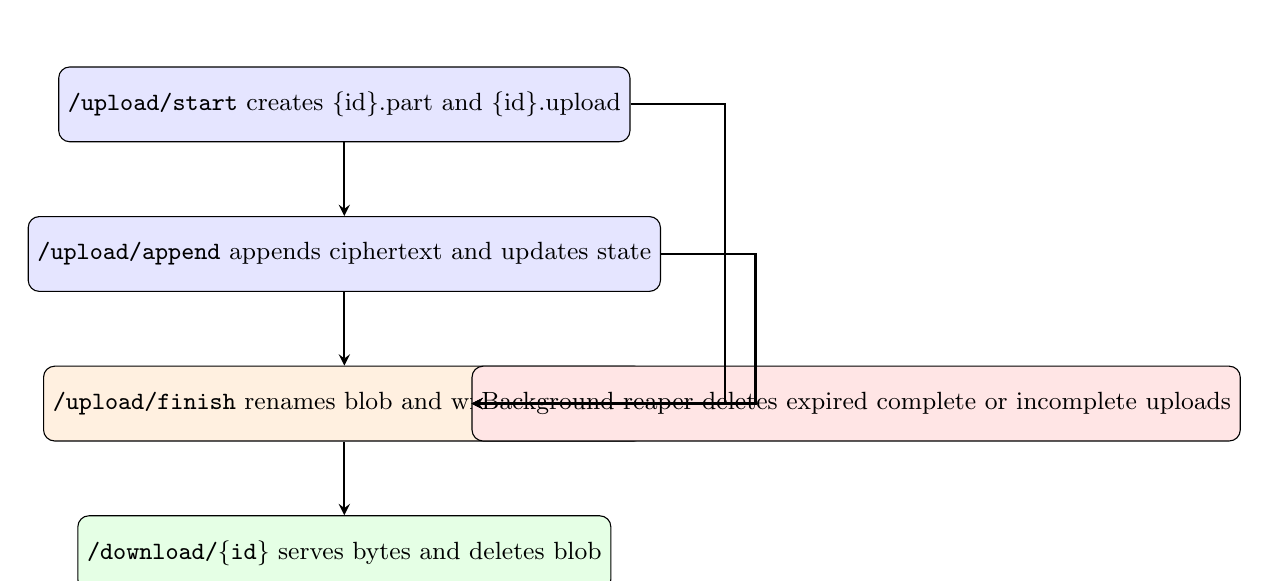
\begin{tikzpicture}[
    node distance=1.9cm,
    box/.style={draw, rounded corners, minimum width=4.2cm, minimum height=0.95cm, align=center, font=\small},
    arr/.style={->, thick, >=stealth}
]
    \node[box, fill=blue!10] (start) {\texttt{/upload/start} creates \{id\}.part and \{id\}.upload};
    \node[box, fill=blue!10, below of=start] (append) {\texttt{/upload/append} appends ciphertext and updates state};
    \node[box, fill=orange!12, below of=append] (finish) {\texttt{/upload/finish} renames blob and writes \{id\}.meta};
    \node[box, fill=green!10, below of=finish] (download) {\texttt{/download/\{id\}} serves bytes and deletes blob};
    \node[box, fill=red!10, right of=finish, xshift=4.6cm] (reap) {Background reaper deletes expired complete or incomplete uploads};

    \draw[arr] (start) -- (append);
    \draw[arr] (append) -- (finish);
    \draw[arr] (finish) -- (download);
    \draw[arr] (start.east) -- ++(1.2,0) |- (reap.west);
    \draw[arr] (append.east) -- ++(1.2,0) |- (reap.west);
    \draw[arr] (finish.east) -- (reap.west);
\end{tikzpicture}
\end{center}

\section{Normal Successful Flow}

\begin{enumerate}
    \item Sender asks the relay for an upload session.
    \item Relay returns ID and upload token.
    \item Sender encrypts and frames the file locally.
    \item Sender issues ordered append requests with the token and chunk index.
    \item Relay appends bytes to the temporary file.
    \item Sender finalizes the upload.
    \item Relay promotes the temp file to a downloadable blob and writes metadata.
    \item Receiver downloads the blob.
    \item Relay deletes the blob immediately after serving it.
    \item Receiver decrypts and verifies the file client-side.
\end{enumerate}

\section{Failure Paths}

Common failure paths in the current implementation include:

\begin{itemize}[leftmargin=1.5cm]
    \item bad HTTP method
    \item missing or invalid token
    \item out-of-order append index
    \item oversize append body
    \item completed upload exceeding global size limit
    \item missing blob on download
    \item rate-limit rejection
    \item stale upload removed by the reaper before completion
\end{itemize}

%==============================================================================
\chapter{Implementation Notes and Current Limitations}
%==============================================================================

\section{Simple by Design}

The relay is intentionally small, which makes it easy to audit and easy to run. That said, the current implementation also has some practical limitations worth recording.

\section{Notable Limitations}

\begin{enumerate}
    \item \textbf{Download reads the full blob into memory.} For larger files, a fully streamed disk-to-socket download path would be more memory-efficient.
    \item \textbf{Rate limiting is in-memory only.} Limits disappear on restart and do not coordinate across multiple relay instances.
    \item \textbf{Delete route prefix mismatch exists in the provided code.} The dispatcher and handler disagree on the expected path prefix.
    \item \textbf{CORS allow-origin is static.} This is simple but requires careful deployment configuration.
    \item \textbf{Metadata is minimal.} That keeps privacy exposure low, but it also means the relay has almost no introspection into stored uploads.
    \item \textbf{Nonce construction should be reviewed carefully.} The protocol helper currently initializes connection IDs to zero in the provided code.
\end{enumerate}

\section{Strengths}

Even with those caveats, the relay has several strong qualities:

\begin{itemize}[leftmargin=1.5cm]
    \item clear upload state machine
    \item exact append ordering enforcement
    \item clean atomic finalization step
    \item straightforward TTL-based garbage collection
    \item file-backed persistence without external dependencies
    \item good request-level logging for debugging
\end{itemize}

%==============================================================================
\chapter{Conclusion}
%==============================================================================

The Zend relay is a compact, practical encrypted blob relay built around a filesystem-backed upload state machine. Its job is to accept opaque encrypted frames, preserve their order, expose the final ciphertext blob for download, and then clean up quickly. The server deliberately avoids deeper responsibilities such as plaintext processing or key management.

From the code provided, the relay already has the core properties needed for a working product prototype: bounded uploads, per-IP limits, upload resumption safety through index checking, background expiry, and simple token-based authorization for upload continuation and deletion. The main areas that still deserve attention are route consistency, download streaming efficiency, and a careful review of protocol nonce handling in the client/format layer.

\vfill
\begin{center}
    \textit{End of document.}
\end{center}

\end{document}
